\documentclass[11pt, oneside]{article}   	% use "amsart" instead of "article" for AMSLaTeX format
\usepackage{geometry}                		% See geometry.pdf to learn the layout options. There are lots.
\geometry{letterpaper}                   		% ... or a4paper or a5paper or ... 
\usepackage{graphicx}				% Use pdf, png, jpg, or eps§ with pdflatex; use eps in DVI mode
								% TeX will automatically convert eps --> pdf in pdflatex		
\usepackage{amssymb}
\usepackage{program}

\title{Assignment 4: Decision Making under Uncertainty and Learning}
\author{Alex Smirnov, Scott Reyes}
\date{May 1, 2017}							

\begin{document}
\maketitle
%\section{}
%\subsection{}
\begin{flushleft}

\section*{Question 1:}
Note: States are referred by their index rather than their state number.\linebreak
Iteration: 0
\begin{center}
\begin{tabular}{|c|c|}
\hline
Node &	Utility \\ \hline
0 &	0.0 \\ \hline
1 &	0.0 \\ \hline
2 &	1.0 \\ \hline
3 &	0.0 \\ \hline
\end{tabular}
\end{center}

Iteration: 1
\begin{center}
\begin{tabular}{|c|c|c|}
\hline
Action & Node &	Utility \\ \hline
2 & 0 &	0.0 \\ \hline
2 & 1 &	0.7200000000000001 \\ \hline
3 & 2 &	1.6480000000000001 \\ \hline
1 & 3 &	1.33488 \\ \hline
\end{tabular}
\end{center}

Iteration: 5
\begin{center}
\begin{tabular}{|c|c|c|}
\hline
Action & Node &	Utility \\ \hline
2 & 0 &	2.337017421689511 \\ \hline
2 & 1 &	2.6655934354214406 \\ \hline
3 & 2 &	3.4750243795365288 \\ \hline
1 & 3 &	3.0622721853782413 \\ \hline
\end{tabular}
\end{center}

Iteration: 15
\begin{center}
\begin{tabular}{|c|c|c|}
\hline
Action & Node &	Utility \\ \hline
2 & 0 &	3.713231422293591 \\ \hline
2 & 1 &	4.176962967443245 \\ \hline
3 & 2 &	4.816810731150936 \\ \hline
1 & 3 &	4.283297765347352 \\ \hline
\end{tabular}
\end{center}

Iteration: 60
\begin{center}
\begin{tabular}{|c|c|c|}
\hline
Action & Node &	Utility \\ \hline
2 & 0 &	3.929362496465146 \\ \hline
2 & 1 &	4.414469642322995 \\ \hline
3 & 2 &	5.027597905122635 \\ \hline
1 & 3 &	4.475114093661598 \\ \hline
\end{tabular}
\end{center}

Iteration: 150
\begin{center}
\begin{tabular}{|c|c|c|}
\hline
Action & Node &	Utility \\ \hline
2 & 0 &	3.9293895701383725 \\ \hline
2 & 1 &	4.414499393612255 \\ \hline
3 & 2 &	5.027624309391853 \\ \hline
1 & 3 &	4.4751381215465855 \\ \hline
\end{tabular}
\end{center}

The implementation used to code value iteration was the Bellman equation. The equation iteratively updates the utility of a node via the maximum of the utility of the best available actions. This value is then discounted and added to the reward before being stored as the next iteration's utility value. The convergence criteria was comparing the maximum change in utility of the current iteration to a maximum error multiplied by the complement of the discount factor expressed in terms of the discount factor. This is essentially to keep iterating until we reach some level of precision in terms of converging with the actual utility. When value iteration is called on the graph with the arguments discount = 0.9, and maxError = .000000000000001, the method iterates 177 times until it reaches convergence. Increasing the discount factor increases the number of iterations needed to reach convergence, and increasing the maximum error allowed deceases the number of iterations needed to reach convergence. The time it takes to call the function on a computer with a CPU: i7-4770k will be around 2 milliseconds for 177 iteration when nothing is printed to the terminal.

\section*{Question 2:}
\subsection*{a}

\subsection*{b}

\subsection*{c}

\section*{Question 3:}
\subsection*{a}

\subsection*{b}

\subsection*{c}

\section*{Question 4:}
\subsection*{a}
Constant offset = 1\\
Class -1 Inputs:\\
(0.1, 1), (0.35, 0.95), (0.7, 0.65), (0.9, 0.45)\\
Class 1 Inputs: \\
(0.1, 0.7), (0.3, 0.55), (0.45, 0.15), (0.6, 0.3)\\
Initial Weights:\\
$w_0 = 0.2$\\
$w_1 = 1$\\
$w_2 = -1$\\
$y=(0.2*1)+((0.1*-1)+(0.35*-0.95)+(0.7*-0.65)+(0.9*-0.45)+(0.1*-0.7)+(0.3*-0.55)+(0.45*-0.15)+(0.6*-0.3))x$\\
$y=0.2+(-0.1-0.3325-0.455-0.405-0.07-0.165-0.0675-0.18)x$\\
$y=-1.775x+0.2$\\
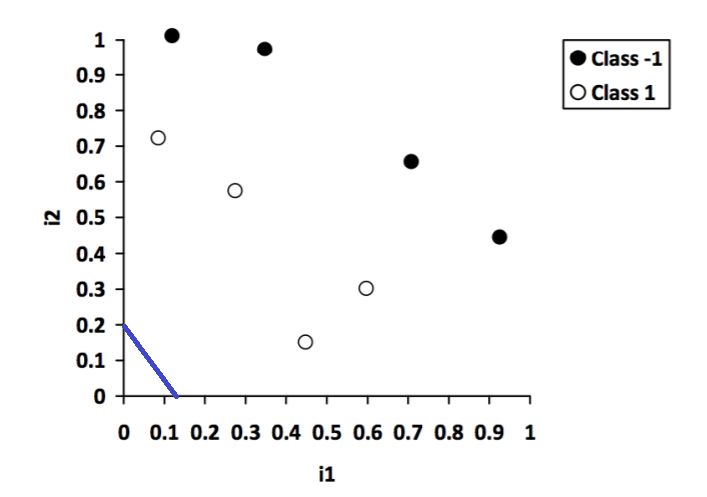
\includegraphics[]{q4_1.png}
\\
4 samples are misclassified after the initial line of separation is placed. Class 1 input (0.1, 0.7) is misclassified, so the weights will be adjusted accordingly.\\
$w_0 = 1$\\
$w_1 = 1$\\
$w_2 = -1$\\
$y=(1*1)+((0.1*-1)+(0.35*-0.95)+(0.7*-0.65)+(0.9*-0.45)+(0.1*-0.7)+(0.3*-0.55)+(0.45*-0.15)+(0.6*-0.3))x$\\
$y=1+(-0.1-0.3325-0.455-0.405-0.07-0.165-0.0675-0.18)x$\\
$y=-1.775x+1$\\
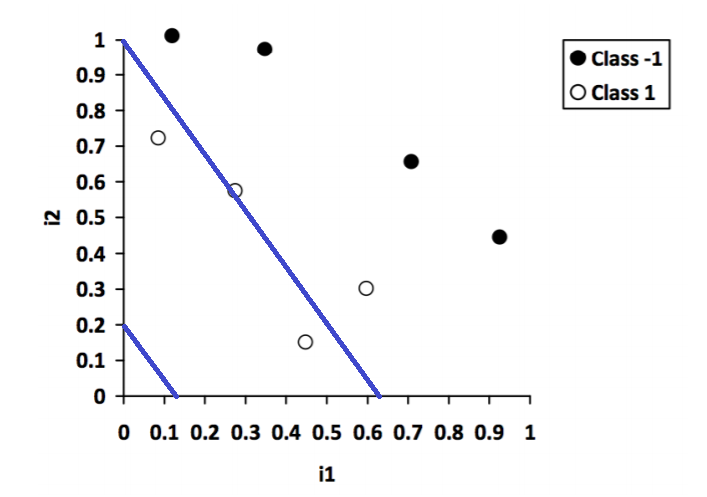
\includegraphics[]{q4_2.png}
\\
2 samples are misclassified after the second line is placed. Class 1 input (0.3, 0.55) is misclassified, so the weights will be adjusted accordingly.\\
$w_0 = 1$\\
$w_1 = 0.8$\\
$w_2 = -1$\\
$y=(1*1)+((0.08*-1)+(0.28*-0.95)+(0.56*-0.65)+(0.72*-0.45)+(0.08*-0.7)+(0.24*-0.55)+(0.36*-0.15)+(0.48*-0.3))x$\\
$y=1+(-0.08-0.266-0.364-0.324-0.056-0.132-0.054-0.144)x$\\
$y=-1.42x+1$\\
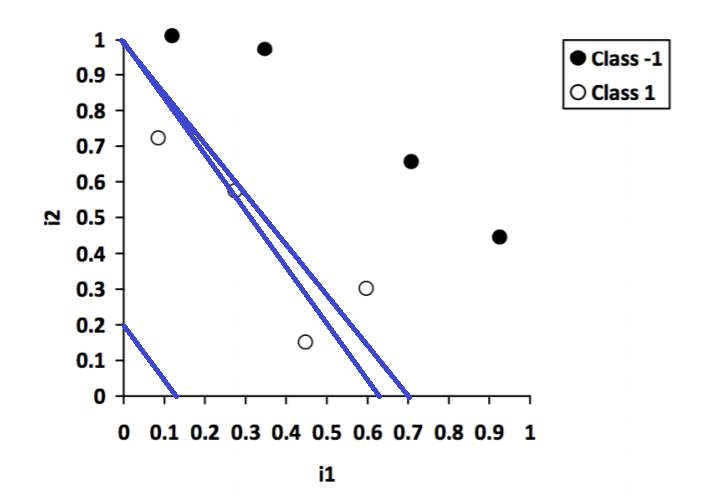
\includegraphics[]{q4_3.png}
\\
1 sample is misclassified after the third line is placed. Class 1 input (0.6, 0.3) is misclassified, so the weights will be adjusted accordingly.\\
$w_0 = 1$\\
$w_1 = 0.5$\\
$w_2 = -1$\\
$y=(1*1)+((0.05*-1)+(0.175*-0.95)+(0.35*-0.65)+(0.45*-0.45)+(0.05*-0.7)+(0.15*-0.55)+(0.225*-0.15)+(0.3*-0.3))x$\\
$y=1+(-0.05-0.16625-0.2275-0.2025-0.035-0.0825-0.03375-0.09)x$\\
$y=-0.8875x+1$\\
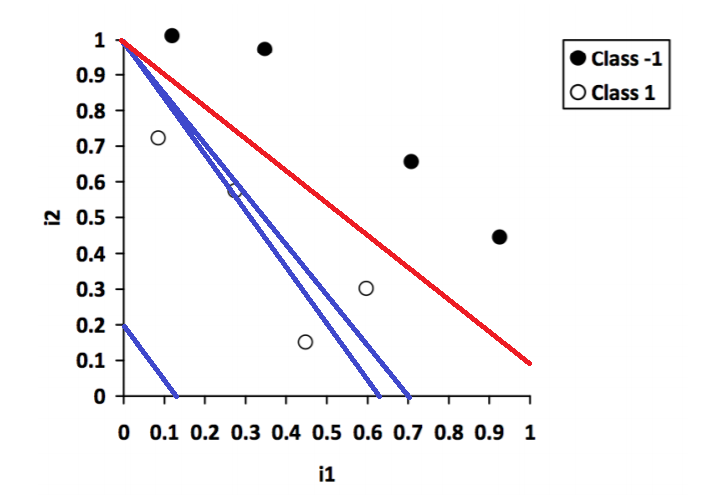
\includegraphics[]{q4_4.png}
No samples are misclassified after the fourth line is placed.\\
\subsection*{b}
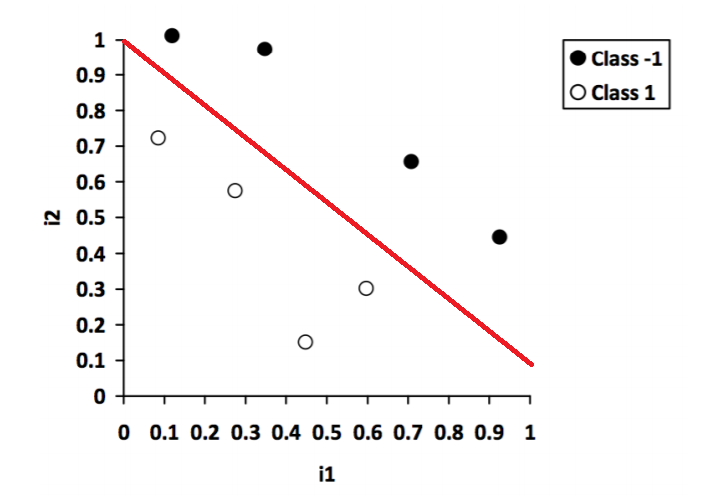
\includegraphics[]{q4_final.png}
\\
This is the final line that achieved perfect classification.\\
$w_0 = 1$\\
$w_1 = 0.5$\\
$w_2 = -1$\\
$y=-0.8875x+1$\\
\subsection*{c}
Constant offset = 1\\
Class -1 Inputs:\\
(0.1), (0.35), (0.7), (0.9)\\
Class 1 Inputs: \\
(0.1), (0.3), (0.45), (0.6)\\
Initial Weights:\\
$w_0 = 1$\\
$w_1 = -0.25$\\
$y=(1*1)+(-0.025-0.0875-0.175-0.225-0.025-0.075-0.1125-0.15)x$\\
$y=-0.875+1$\\
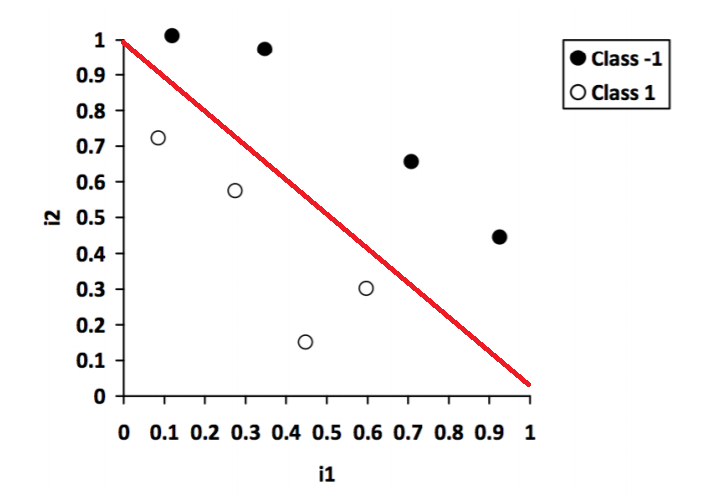
\includegraphics[]{q4_c_final.png}
\\
The error for this input space separation is 0 because all of the inputs are correctly classified.\\
\section*{Question 5:}
\subsection*{a}
The minimum error that can be reached with a single perceptron for this classification task is 2, which means 2 points will be classified incorrectly no matter how much learning the perceptron does.\\
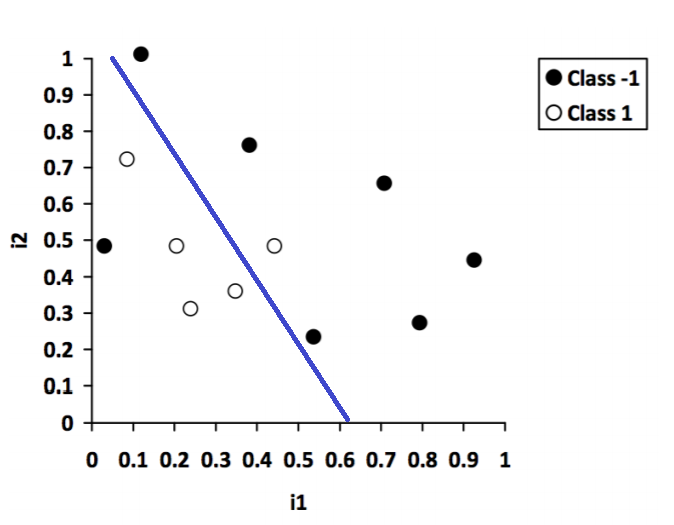
\includegraphics[]{q5_line_1.png} \\
\subsection*{b}
To correctly classify all of these point, we need at least 3 linear separators and one node in the next layer to combine the output of those 3 linear separators. This final node accepts the last two perceptrons as given before inverting the third one' class to be 1. Thus a positive signal will be output only when the first perception returns a class -1 and the last two return a class 1.
the linear separator is given in the form of $w_{1}*x_{1}+w_{2}*x_{2}+w_{3}*x_{3}=0$
\begin{center}
\begin{tabular}{|c|c|c|c|c|}
\hline
Layer & Node & w1 &	w2 & w3 \\ \hline
1 & 0 & -.8 & 1 & .5 \\ \hline
1 & 1 & 0 & -1 & .9 \\ \hline
1 & 2 &	-.8 & 1 & 3 \\ \hline
2 & 3 &	-1 & 1 & 1 \\ \hline
\end{tabular}
\end{center}
Final result of the multilayer perceptron line drawing: \\
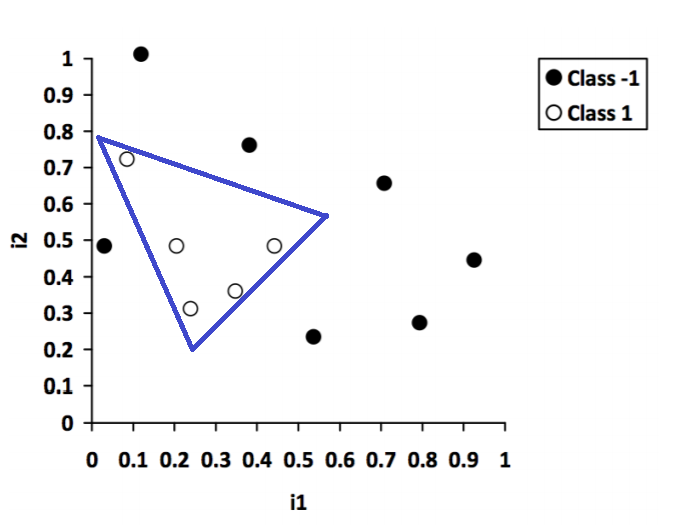
\includegraphics[]{q5_mlp.png}
%need to finish multilayer perceptron network

\end{flushleft}
\end{document}  